%++++++++++++++++++++++++++++++++++++++++
\documentclass[article, 12pt]{article}
\usepackage{float}
\usepackage{setspace}
\usepackage{tabu} % extra features for tabular environment
\usepackage{amsmath}  % improve math presentation
\usepackage{graphicx} % takes care of graphic including machinery
\usepackage[margin=1in]{geometry} % decreases margins
\usepackage{cite} % takes care of citations
\usepackage[final]{hyperref} % adds hyper links inside the generated pdf file
\usepackage{tikz}
\usepackage{caption} 
\usepackage{fancyhdr}
\usepackage{amssymb} % symbols like /therefore
\usepackage{amsthm} % proofs
\usepackage{enumerate} % lettered lists
\usepackage{mathtools} % macros
\usepackage[all]{xy} % for diagrams
\usepackage{tkz-graph}
\usetikzlibrary{knots}
\usepackage{xcolor}
\usetikzlibrary{scopes}
% \usepackage{xcolor} \pagecolor[rgb]{0.12549019607,0.1294117647,0.13725490196} \color[rgb]{0.82352941176,0.76862745098,0.62745098039} % dark theme
\theoremstyle{definition}
\newtheorem{example}{Example}[subsubsection]
\newtheorem*{remark}{Remark}
\newtheorem{theorem}{Theorem}[subsubsection]
\newtheorem{definition}{Definition}[subsubsection]
\newtheorem{corollary}{Corollary}[subsubsection]
\hypersetup{
	colorlinks=false,      % false: boxed links; true: colored links
	linkcolor=blue,        % color of internal links
	citecolor=blue,        % color of links to bibliography
	filecolor=magenta,     % color of file links
	urlcolor=blue         
}
\usepackage{physics}
\usepackage{siunitx}
\usepackage{tikz,pgfplots}
\usepackage[outline]{contour} % glow around text
\usetikzlibrary{calc}
\usetikzlibrary{angles,quotes} % for pic
\usetikzlibrary{arrows.meta}
\tikzset{>=latex} % for LaTeX arrow head
\contourlength{1.2pt}

\colorlet{xcol}{blue!70!black}
\colorlet{vcol}{green!60!black}
\colorlet{myred}{red!70!black}
\colorlet{myblue}{blue!70!black}
\colorlet{mygreen}{green!70!black}
\colorlet{mydarkred}{myred!70!black}
\colorlet{mydarkblue}{myblue!60!black}
\colorlet{mydarkgreen}{mygreen!60!black}
\colorlet{acol}{red!50!blue!80!black!80}
\tikzstyle{CM}=[red!40!black,fill=red!80!black!80]
\tikzstyle{xline}=[xcol,thick,smooth]
\tikzstyle{mass}=[line width=0.6,red!30!black,fill=red!40!black!10,rounded corners=1,
                  top color=red!40!black!20,bottom color=red!40!black!10,shading angle=20]
\tikzstyle{faded mass}=[dashed,line width=0.1,red!30!black!40,fill=red!40!black!10,rounded corners=1,
                        top color=red!40!black!10,bottom color=red!40!black!10,shading angle=20]
\tikzstyle{rope}=[brown!70!black,very thick,line cap=round]
\def\rope#1{ \draw[black,line width=1.4] #1; \draw[rope,line width=1.1] #1; }
\tikzstyle{force}=[->,myred,very thick,line cap=round]
\tikzstyle{velocity}=[->,vcol,very thick,line cap=round]
\tikzstyle{Fproj}=[force,myred!40]
\tikzstyle{myarr}=[-{Latex[length=3,width=2]},thin]
\def\tick#1#2{\draw[thick] (#1)++(#2:0.12) --++ (#2-180:0.24)}
\DeclareMathOperator{\sn}{sn}
\DeclareMathOperator{\cn}{cn}
\DeclareMathOperator{\dn}{dn}
\def\N{80} % number of samples in plots


\usepackage{titling}
\renewcommand\maketitlehooka{\null\mbox{}\vfill}
\renewcommand\maketitlehookd{\vfill\null}
\usepackage{siunitx} % units
\usepackage{verbatim} 
\newcommand{\courseNumber}{MATH 1700}
\newcommand{\courseName}{Ideas in Mathematics}
\newcommand{\professor}{Professor Rimmer}
\newcommand{\psetName}{Worksheet 10: Introduction to Graphs First Submission}
\newcommand{\dueDate}{Due: April 10, 2023}
\newcommand{\name}{Denny Cao}
\pagestyle{fancy}
\fancyhf{}% clears all header and footer fields
\fancyfoot[C]{--~\thepage~--}
\renewcommand*{\headrulewidth}{0.4pt}
\renewcommand*{\footrulewidth}{0pt}
\lhead{\name}
\chead{\courseNumber: \courseName}
\rhead{\professor}

% new theorem for questions and answers

\newtheorem{question}{Question}

\newtheorem{answer}{Answer}

\fancypagestyle{plain}{%
  \fancyhf{}% clears all header and footer fields
  \fancyfoot[C]{--~\thepage~--}%
  \renewcommand*{\headrulewidth}{0pt}%
  \renewcommand*{\footrulewidth}{0pt}%
}

% Shortcuts
\DeclarePairedDelimiter\ceil{\lceil}{\rceil} % ceil function
\DeclarePairedDelimiter\floor{\lfloor}{\rfloor} % floor function

\DeclarePairedDelimiter\paren{(}{)} % parenthesis

\newcommand{\df}{\displaystyle\frac} % displaystyle fraction
\newcommand{\qeq}{\overset{?}{=}} % questionable equality

\newcommand{\Mod}[1]{\;\mathrm{mod}\; #1} % modulo operator

\newcommand{\comp}{\circ} % composition

% Sets
\DeclarePairedDelimiter\set{\{}{\}}
\newcommand{\unite}{\cup}
\newcommand{\inter}{\cap}

\newcommand{\reals}{\mathbb{R}} % real numbers: textbook is Z^+ and 0
\newcommand{\ints}{\mathbb{Z}}
\newcommand{\nats}{\mathbb{N}}
\newcommand{\rats}{\mathbb{Q}}

\newcommand{\degree}{^\circ}

% Counting
\newcommand\perm[2][^n]{\prescript{#1\mkern-2.5mu}{}P_{#2}}
\newcommand\comb[2][^n]{\prescript{#1\mkern-0.5mu}{}C_{#2}}

% Relations
\newcommand{\rel}{\mathcal{R}} % relation

\setlength\parindent{0pt}

% Directed Graphs
\usetikzlibrary{arrows}
\tikzset{vertex/.style = {shape=circle,draw,minimum size=2em}}
\tikzset{svertex/.style = {shape=circle,draw,minimum size=.05em,font=\tiny}}
\tikzset{edge/.style = {->,> = latex'}}
\tikzset{dedge/.style = {-> = latex'}}
\tikzset{dot/.style={inner sep=1.5pt,circle,draw,fill}}

% Contradiction
\newcommand{\contradiction}{{\hbox{%
    \setbox0=\hbox{$\mkern-3mu\times\mkern-3mu$}%
    \setbox1=\hbox to0pt{\hss$\times$\hss}%
    \copy0\raisebox{0.5\wd0}{\copy1}\raisebox{-0.5\wd0}{\box1}\box0
}}}

% Sign Charts
\newdimen\tcolw \tcolw=2.5em % the column width
\edef\ecatcode{\catcode`&=\the\catcode`&\relax}\catcode`&=4
\def\sgchart#1#2{\vbox{\offinterlineskip\halign{\hfil##\quad&##\hfil\crcr\sgchartA#2,:,%
   \omit\sgchartR&\kern.2pt\sgchartS{.5\tcolw}\relax\sgchartE#1,\relax,%
   \sgchartS{.5\tcolw}\relax\cr
   \noalign{\kern2pt}&\def~{}\kern.5\tcolw\sgchartD#1,\relax,\cr}}}
\def\sgchartA#1:#2,{\cr\ifx,#1,\else $#1$&\sgchartB#2{}\expandafter\sgchartA\fi}
\def\sgchartB#1{\hbox to\tcolw{\hss$#1$\hss}\sgchartC}
\def\sgchartC#1{\ifx,#1,\else
   \strut\vrule\kern-.4pt\hbox to\tcolw{\hss$#1$\hss}\expandafter\sgchartC\fi}
\def\sgchartD#1#2,{\ifx\relax#1\else\hbox to\tcolw{\hss$#1#2$\hss}\expandafter\sgchartD\fi}
\def\sgchartE#1#2,{\ifx\relax#1\else
    \ifx~#1\sgchartS\tcolw\circ \else\sgchartS\tcolw\bullet\fi \expandafter\sgchartE\fi}
\def\sgchartR{\leaders\vrule height2.8pt depth-2.4pt\hfil}
\def\sgchartS#1#2{\hbox to#1{\kern-.2pt\sgchartR \ifx\relax#2\else
   \kern-.7pt$#2$\kern-.7pt\sgchartR\fi\kern-.2pt}}
\ecatcode
%++++++++++++++++++++++++++++++++++++++++
% title stuff

\makeatletter
\renewcommand{\maketitle}{\bgroup\setlength{\parindent}{0pt}
    \begin{flushleft}
        \textbf{\@title} \\ \vskip0.2cm
        \begingroup
            \fontsize{14pt}{12pt}\selectfont
            \courseNumber: \courseName 
            \vskip0.3cm 
            \professor
        \endgroup \vskip0.3cm
        \dueDate \hfill\rlap{}\bf{\name} \\ \vskip0.1cm
        \hrulefill
    \end{flushleft}\egroup 
}
\makeatother

\title{\Large\bf{\psetName}}

\begin{document}
    \maketitle
    \thispagestyle{plain}
    \section{Warm-Up}
    Bulbasaur (B), Charmander (C), Squirtle (S), and Pikachu (P) are battling at the same gym. (``Y'' indicates that a pair faced off, and ``N'' means that they didn't):
    \begin{figure}[H]
        \centering
        \begin{tabular}{|c|c|c|c|c|}
            \hline
              & B & C & S & P \\
            \hline
            B & N & Y & Y & Y \\
            C & Y & N & Y & N \\
            S & Y & Y & N & N \\
            P & Y & N & N & N \\
            \hline
        \end{tabular}
    \end{figure}
    % Question 1
    \begin{question}
        Model the information from the table with a graph. What do the vertices and edges represent?
    \end{question}
    % Answer 1
    \begin{answer} The vertices represent the Pokemon, and the edges represent the battles. 
        \begin{figure}[H]
            \centering
            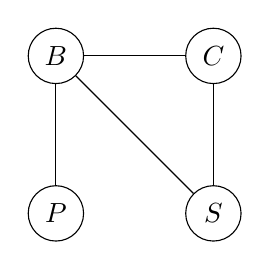
\begin{tikzpicture}
                \node[vertex] (B) at (0,0) {$B$};
                \node[vertex] (C) at (2,0) {$C$};
                \node[vertex] (S) at (2,-2) {$S$};
                \node[vertex] (P) at (0,-2) {$P$};
                \draw (B) -- (C);
                \draw (B) -- (S);
                \draw (B) -- (P);
                \draw (C) -- (S);
            \end{tikzpicture}
        \end{figure}
    \end{answer}
    % Question 2
    \begin{question}
        Write down the degree of each of the vertices in your graph. What does the degree of a vertex represent?
    \end{question}
    % Answer 2 
    \begin{answer} The degree of a vertex is the number of edges incident on it. In this case, it means the number of Pokemon that a Pokemon has battled.
        \begin{figure}[H]
            \centering
            \begin{tabular}{|c|c|}
                \hline
                Vertex & Degree \\
                \hline
                $B$ & 3 \\
                $C$ & 2 \\
                $S$ & 2 \\
                $P$ & 1 \\
                \hline
            \end{tabular}
        \end{figure}
    \end{answer}
    % Question 3
    \begin{question}
        Is your graph connected? Does it have cycles?
    \end{question}
    % Answer 3
    \begin{answer}
        The graph is connected because there exists a path between every pair of vertices. A cycle is a path that starts and ends at the same vertex. In this graph, there exists a cycle: $B, C, S, B$.
    \end{answer}
    \section{Spanning Trees}
    % Question 4
    \begin{question}
        You have four trees in a level area in your garden. You would like to dig an irrigation system connecting the trees, so that when you pour water near one tree, the water flows and reaches all of the other trees. Here is a graph whose vertices represent the trees, and whose edges represent each of the possible ways to connect two trees with a ditch:
        \begin{figure}[H]
            \centering
            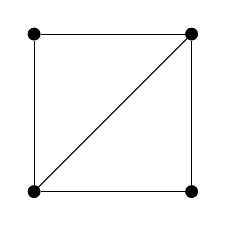
\begin{tikzpicture}
                \node[dot] (A) at (0,0) {};
                \node[dot] (B) at (2,0) {};
                \node[dot] (C) at (0,-2) {};
                \node[dot] (D) at (2,-2) {};

                \draw (A) -- (B);
                \draw (B) -- (D);
                \draw (D) -- (C);
                \draw (C) -- (A);
                \draw (C) -- (B);
            \end{tikzpicture}
        \end{figure}
        Assuming that all of the edges are equally labor-intensive to dig, and that you don't want to do unnecessary work, which of the following plans, where the edges to be dug are colored red, is best for your purposes, and why? Try to use as much of our new graph terminology as you can!
        \begin{figure}[H]
            \centering
            \begin{minipage}[b]{0.2\linewidth}
                \caption*{Plan 1:}
                \centering
                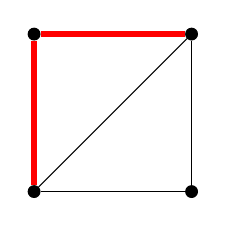
\begin{tikzpicture}
                    \node[dot] (A) at (0,0) {};
                    \node[dot] (B) at (2,0) {};
                    \node[dot] (C) at (0,-2) {};
                    \node[dot] (D) at (2,-2) {};

                    \draw[red, line width=0.8mm] (A) -- (B);
                    \draw (B) -- (D);
                    \draw (D) -- (C);
                    \draw[red, line width=0.8mm] (C) -- (A);
                    \draw (C) -- (B);

                \end{tikzpicture}
            \end{minipage}
            \begin{minipage}[b]{0.2\linewidth}
                \caption*{Plan 2:}
                \centering
                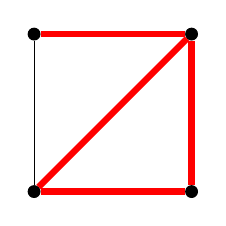
\begin{tikzpicture}
                    \node[dot] (A) at (0,0) {};
                    \node[dot] (B) at (2,0) {};
                    \node[dot] (C) at (0,-2) {};
                    \node[dot] (D) at (2,-2) {};

                    \draw[red, line width=0.8mm] (A) -- (B);
                    \draw[red, line width=0.8mm] (B) -- (D);
                    \draw[red, line width=0.8mm] (D) -- (C);
                    \draw (C) -- (A);
                    \draw[red, line width=0.8mm] (C) -- (B);
                \end{tikzpicture}
            \end{minipage}
            \begin{minipage}[b]{0.2\linewidth}
                \caption*{Plan 3:}
                \centering
                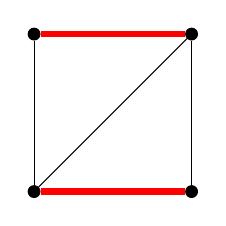
\begin{tikzpicture}
                    \node[dot] (A) at (0,0) {};
                    \node[dot] (B) at (2,0) {};
                    \node[dot] (C) at (0,-2) {};
                    \node[dot] (D) at (2,-2) {};

                    \draw[red, line width=0.8mm] (A) -- (B);
                    \draw (B) -- (D);
                    \draw[red, line width=0.8mm] (D) -- (C);
                    \draw (C) -- (A);
                    \draw (C) -- (B);
                \end{tikzpicture}
            \end{minipage}
            \begin{minipage}[b]{0.2\linewidth}
                \caption*{Plan 4:}
                \centering
                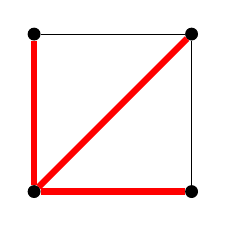
\begin{tikzpicture}
                    \node[dot] (A) at (0,0) {};
                    \node[dot] (B) at (2,0) {};
                    \node[dot] (C) at (0,-2) {};
                    \node[dot] (D) at (2,-2) {};

                    \draw (A) -- (B);
                    \draw (B) -- (D);
                    \draw[red, line width=0.8mm] (D) -- (C);
                    \draw[red, line width=0.8mm] (C) -- (A);
                    \draw[red, line width=0.8mm] (C) -- (B);
                \end{tikzpicture}
            \end{minipage}
        \end{figure}
    \end{question}
    % Answer 4
    \begin{answer}
        Plan 4 is the best plan, because it is a spanning tree. A spanning tree is a subgraph of a graph that connects all of the vertices, and has no cycles. Our proposed plan must be a spanning tree because we want to connect all of the trees. Plan 1 is not a spanning tree because it doesn't connect all of the trees. Plan 2 has a subgraph that is a spanning tree, but the plan itself does unnecessary work by creating a cycle. Plan 3 is not a spanning tree because it doesn't connect all of the trees. Thus, Plan 4 is the best plan.
    \end{answer}
    % Question 5 
    \begin{question}
        Draw three new plans for digging that are equally sensible as the one you chose in the previous problem. What do these ``sensible'' plans have in common, as graphs?
    \end{question}
    % Answer 5
    \begin{answer} They all have to be spanning trees.
        \begin{figure}[H]
            \centering
            \begin{minipage}[b]{0.2\linewidth}
                \caption*{New Plan 1:}
                \centering
                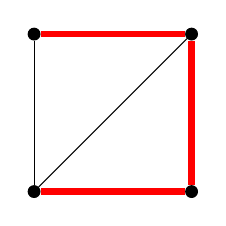
\begin{tikzpicture}
                    \node[dot] (A) at (0,0) {};
                    \node[dot] (B) at (2,0) {};
                    \node[dot] (C) at (0,-2) {};
                    \node[dot] (D) at (2,-2) {};

                    \draw[red, line width=0.8mm] (A) -- (B);
                    \draw[red, line width=0.8mm] (B) -- (D);
                    \draw[red, line width=0.8mm] (D) -- (C);
                    \draw (C) -- (A);
                    \draw (C) -- (B);
                \end{tikzpicture}
            \end{minipage}
            \begin{minipage}[b]{0.2\linewidth}
                \caption*{New Plan 2:}
                \centering
                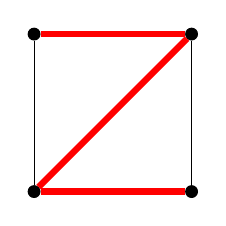
\begin{tikzpicture}
                    \node[dot] (A) at (0,0) {};
                    \node[dot] (B) at (2,0) {};
                    \node[dot] (C) at (0,-2) {};
                    \node[dot] (D) at (2,-2) {};

                    \draw[red, line width=0.8mm] (A) -- (B);
                    \draw (B) -- (D);
                    \draw[red, line width=0.8mm] (D) -- (C);
                    \draw (C) -- (A);
                    \draw[red, line width=0.8mm] (C) -- (B);
                \end{tikzpicture}
            \end{minipage}
            \begin{minipage}[b]{0.2\linewidth}
                \caption*{New Plan 3:}
                \centering
                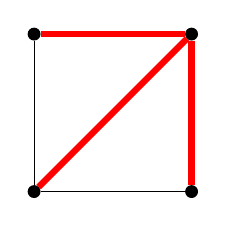
\begin{tikzpicture}
                    \node[dot] (A) at (0,0) {};
                    \node[dot] (B) at (2,0) {};
                    \node[dot] (C) at (0,-2) {};
                    \node[dot] (D) at (2,-2) {};

                    \draw[red, line width=0.8mm] (A) -- (B);
                    \draw[red, line width=0.8mm] (B) -- (D);
                    \draw (D) -- (C);
                    \draw (C) -- (A);
                    \draw[red, line width=0.8mm] (C) -- (B);
                \end{tikzpicture}
            \end{minipage}
        \end{figure}
    \end{answer}
    \section{Matching Problems}
    In the next three problems, imagine you're trying to assign tasks to a group of people completing a project. The people are named $A,B,C,$ and $D$, and the tasks they need to perform are labeled 1,2,3, and 4. Every person needs to be assigned exactly one task, and every task needs to get done.
    % Question 6
    \begin{question}
        In the scenarios depicted by the following two graphs, there is an edge between a person ($A, B, C,$ or $D$) and a task (1, 2, 3, or 4) if that person knows how to do that task. (For instance, Person $A$ in Scenario 1 knows how to do tasks 1 and 2, but doesn't know how to do tasks 3 or 4.)
        \\[12pt]
        For each scenario, determine whether there is an acceptable way to assign people to tasks (everyone must be assigned to exactly one task, all tasks must get done, and a person can only be assigned to a task that they know how to do). If there is a way, exhibit one (this is called a \textit{matching} for the graph). If there isn't, carefully explain why not.
        \begin{figure}[H]
            \centering
            \begin{minipage}[b]{0.4\linewidth}
                \caption*{Scenario 1:}
                \centering
                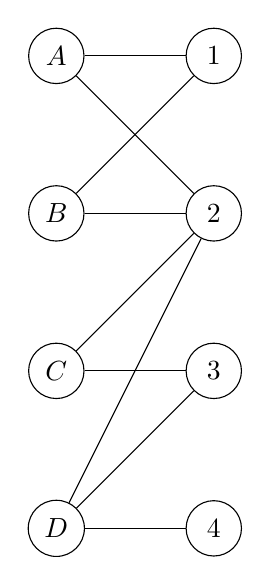
\begin{tikzpicture}
                    \node[vertex] (A) at (0,0) {$A$};
                    \node[vertex] (B) at (0,-2) {$B$};
                    \node[vertex] (C) at (0,-4) {$C$};
                    \node[vertex] (D) at (0,-6) {$D$};
                    
                    \node[vertex] (1) at (2,0) {$1$};
                    \node[vertex] (2) at (2,-2) {$2$};
                    \node[vertex] (3) at (2,-4) {$3$};
                    \node[vertex] (4) at (2,-6) {$4$};

                    \draw (A) -- (1);
                    \draw (A) -- (2);
                    \draw (B) -- (1);
                    \draw (B) -- (2);
                    \draw (C) -- (2);
                    \draw (C) -- (3);
                    \draw (D) -- (2);
                    \draw (D) -- (3);
                    \draw (D) -- (4);
                \end{tikzpicture}
            \end{minipage}
            \begin{minipage}[b]{0.4\linewidth}
                \caption*{Scenario 2:}
                \centering
                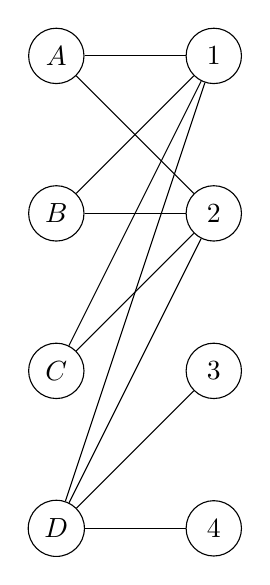
\begin{tikzpicture}
                    \node[vertex] (A) at (0,0) {$A$};
                    \node[vertex] (B) at (0,-2) {$B$};
                    \node[vertex] (C) at (0,-4) {$C$};
                    \node[vertex] (D) at (0,-6) {$D$};
                    
                    \node[vertex] (1) at (2,0) {$1$};
                    \node[vertex] (2) at (2,-2) {$2$};
                    \node[vertex] (3) at (2,-4) {$3$};
                    \node[vertex] (4) at (2,-6) {$4$};

                    \draw (A) -- (1);
                    \draw (A) -- (2);
                    \draw (B) -- (1);
                    \draw (B) -- (2);
                    \draw (C) -- (1);
                    \draw (C) -- (2);
                    \draw (D) -- (1);
                    \draw (D) -- (2);
                    \draw (D) -- (3);
                    \draw (D) -- (4);
                \end{tikzpicture}
            \end{minipage}
        \end{figure}
    \end{question}
    % Answer 6
    \begin{answer} \ \\
        \textbf{Scenario 1:} 
        \begin{proof}
            There is an acceptable way to assign people to tasks. One such way is:
            \begin{figure}[H]
                \centering
                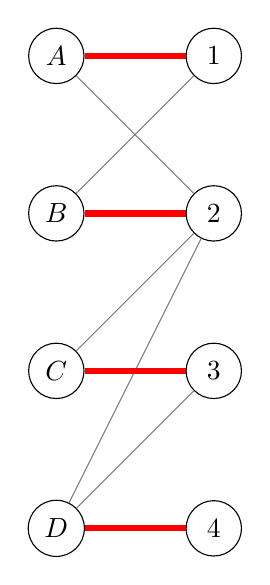
\begin{tikzpicture}
                    \node[vertex] (A) at (0,0) {$A$};
                    \node[vertex] (B) at (0,-2) {$B$};
                    \node[vertex] (C) at (0,-4) {$C$};
                    \node[vertex] (D) at (0,-6) {$D$};
                    
                    \node[vertex] (1) at (2,0) {$1$};
                    \node[vertex] (2) at (2,-2) {$2$};
                    \node[vertex] (3) at (2,-4) {$3$};
                    \node[vertex] (4) at (2,-6) {$4$};

                    \draw[red, line width=0.8mm] (A) -- (1);
                    \draw[black!50] (A) -- (2);
                    \draw[black!50] (B) -- (1);
                    \draw[red, line width=0.8mm] (B) -- (2);
                    \draw[black!50] (C) -- (2);
                    \draw[black!50] (D) -- (2);
                    \draw[black!50] (D) -- (3);
                    \draw[red, line width=0.8mm] (C) -- (3);
                    \draw[red, line width=0.8mm] (D) -- (4);
                \end{tikzpicture}
            \end{figure}
        \end{proof}
        \textbf{Scenario 2:} \begin{proof}
            There is no acceptable way to assign people to tasks. Task 3 and 4 can only be done by $D$, but $D$ can only do one task. Therefore, there is no way to assign people to tasks.
        \end{proof}
    \end{answer}
    % Question 7
    \begin{question}
        The graphs of the sort depicted (i.e., graphs depicting which people in a group of four can do which of four tasks) are called \textit{bipartite}. How does the term \textit{bipartite} reflect the structure of these graphs?
    \end{question}
    % Answer 7
    \begin{answer}
        These graphs can be partitioned into two sets, $V_1$ and $V_2$, such that every edge connects a vertex in $V_1$ to a vertex in $V_2$ and no vertex within the same partition is connected to another vertex within the same partition. In the case of matching, $V_1$ is matched to $V_2$, and people cannot be matched to other people just as tasks cannot be matched to other tasks.
    \end{answer}
    % Question 8
    \begin{question}
        Draw two new graphs like those from Problem 6 (i.e, your graphs should correspond to some possible situation in which each person in the group $A, B, C, D$, knows how to perform some subset of the tasks 1,2,3, and 4). Include one graph in which there is no acceptable way to match people to tasks, and another in which there is a way. Can you name a concrete structural characteristic such a graph might have that would \textit{guarentee} that there is no acceptable way to match people to tasks?
    \end{question}
    % Answer 8
    \begin{answer} A graph that does not have a matching does not satisfy Hall's condition in Hall's Marriage Theorem. Let this graph $G$ be a bipartite graph with $V_1$ and $V_2$ as the two partitions such that $|V_1| \leq |V_2|$. Then, $G$ does not have a matching if and only if, for some $S \subseteq V_1$, $|S| > |N(S)|$, where $N(S)$ is the set of neighbors of $S$. 
        \begin{figure}[H]
            \centering
            \begin{minipage}[b]{0.4\linewidth}
                \caption*{Matching $K_{4,4}$:}
                \centering
                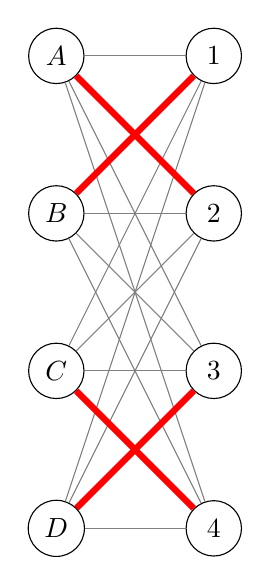
\begin{tikzpicture}
                    \node[vertex] (A) at (0,0) {$A$};
                    \node[vertex] (B) at (0,-2) {$B$};
                    \node[vertex] (C) at (0,-4) {$C$};
                    \node[vertex] (D) at (0,-6) {$D$};
                    
                    \node[vertex] (1) at (2,0) {$1$};
                    \node[vertex] (2) at (2,-2) {$2$};
                    \node[vertex] (3) at (2,-4) {$3$};
                    \node[vertex] (4) at (2,-6) {$4$};

                    \draw[black!50] (A) -- (1);
                    \draw[black!50] (A) -- (3);
                    \draw[black!50] (A) -- (4);
                    \draw[black!50] (B) -- (2);
                    \draw[black!50] (B) -- (3);
                    \draw[black!50] (B) -- (4);
                    \draw[black!50] (C) -- (1);
                    \draw[black!50] (C) -- (2);
                    \draw[black!50] (C) -- (3);
                    \draw[black!50] (D) -- (1);
                    \draw[black!50] (D) -- (2);
                    \draw[black!50] (D) -- (4);
                    \draw[red, line width=0.8mm] (A) -- (2);
                    \draw[red, line width=0.8mm] (B) -- (1);
                    \draw[red, line width=0.8mm] (C) -- (4);
                    \draw[red, line width=0.8mm] (D) -- (3);
                \end{tikzpicture}
            \end{minipage}
            \begin{minipage}[b]{0.4\linewidth}
                \caption*{No Matching:}
                \centering
                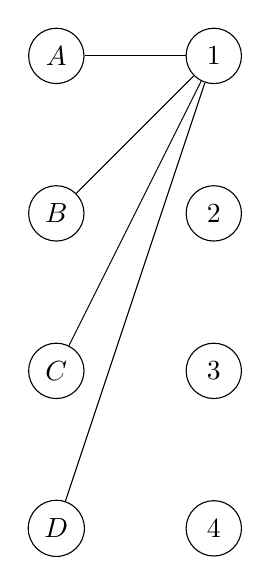
\begin{tikzpicture}
                    \node[vertex] (A) at (0,0) {$A$};
                    \node[vertex] (B) at (0,-2) {$B$};
                    \node[vertex] (C) at (0,-4) {$C$};
                    \node[vertex] (D) at (0,-6) {$D$};
                    
                    \node[vertex] (1) at (2,0) {$1$};
                    \node[vertex] (2) at (2,-2) {$2$};
                    \node[vertex] (3) at (2,-4) {$3$};
                    \node[vertex] (4) at (2,-6) {$4$};

                    \draw (A) -- (1);
                    \draw (B) -- (1);
                    \draw (C) -- (1);
                    \draw (D) -- (1);
                \end{tikzpicture}
            \end{minipage}
        \end{figure}
    \end{answer}
    \section{Social Networks}
    \begin{question}
        Consider the following social network, where each vertex is a Simpsons character, and each edge represents a friendship between characters.
    \end{question}
\end{document} 
